\chapter{{\en {PELOMA: A Personalized News Recommendation System}}}

Στην ενότητα αυτή θα παρουσιάσουμε την διεπαφή χρήστη. 
Η διεπαφή αποτελεί έναν σημαντικό διαμεσολαβητή μεταξύ συστήματος και χρήστη. 
Μέσω της διεπαφής ο χρήστης έχει την δυνατότητα να επικοινωνήσει με το σύστημα, 
δηλαδή να δώσει τα δεδομένα του σε αυτό και να πάρει αποτελέσματα από αυτό. \\

Για να μπορέσει να λειτουργήσει η εφαρμογή θα πρέπει να εκτελεστούν μια φορά τα απαραίτητα
υποσυστήματα, η λειτουργία των οποίων έχει αναλυθεί εκτενώς στο Κεφάλαιο 2:

\begin{itemize}
\item \textbf{Υποσύστημα Δημιουργίας Βάσης Δεδομένων και Καταχώρησης Πληροφορίας} \\
Το υποσύστημα αυτό θα δημιουργήσει τη βάση δεδομένων και θα καταχωρήσει την απαραίτητη 
για τα επόμενα υποσυστήματα πληροφορία σχετικά με τα άρθρα. 

\item \textbf{Υποσύστημα Ομαδοποίησης Ειδησεογραφικών Άρθρων} \\
Στο υποσύστημα αυτό προβαίνουμε σε ομαδοποίηση των ειδησεογραφικών άρθρων που βρίσκονται 
αποθηκευμένα στη βάση δεδομένων σε κατηγορίες {\en {(clusters)}}, 
ομαδοποίηση των ειδησεογραφικών άρθρων εντός των {\en {clusters}} σε ομάδες {\en {(groups)}}, 
καθώς και σε εντοπισμό ειδησεογραφικών θεμάτων μέσω πιθανοτικών μοντέλων θεμάτων 
για κάθε {\en {cluster, group}} και μεμονωμένο άρθρο της συλλογής. 
Επιπρόσθετα, κάνουμε εξαγωγή ονοματισμένων οντοτήτων για κάθε άρθρο.
Όλη η παραχθείσα νέα πληροφορία αποθηκεύεται στη βάση δεδομένων. 
\end{itemize}

\newpage
Παρακάτω παρουσίαζουμε το περιβάλλον της διεπαφής: \\

\begin{figure}[!ht] \centering
\centerline{
    
\includegraphics[scale=0.45]{static/figures/peloma/start.png}}
    \caption{Αρχική εικόνα περιβάλλοντος διεπαφής.}
    \label{}
\end{figure} 

\begin{figure}[!ht] \centering
\centerline{
    
\includegraphics[scale=0.46]{static/figures/peloma/loading.png}}
    \caption{Αναμονή για δημιουργία προφίλ αποθηκευμένων χρηστών και άρθρων.}
    \label{}
\end{figure} 

% Όπως έχουμε αναφέρει, κατά τη δημιουργία της βάσης δεδομένων καταχωρήσαμε και μία λίστα χρηστών μαζί με το αναγνωστικό τους ιστορικό. \\
Αρχικά, μέσω του κουμπιού {\en {Start!}} δημιουργούμε κάποια έτοιμα προφίλ, 
τόσο για τους αποθηκευμένους χρήστες, όσο και για τα άρθρα που βρίσκονται στο ιστορικό τους, 
πριν επιτρέψουμε σε ένα νέο χρήστη να εισέλθει στο σύστημα. 
Η αναγκαιότητα δημιουργίας έτοιμων προφίλ χρηστών προκύπτει από την απαίτηση του συστήματος για εμπλουτισμό 
κάθε προφίλ χρήστη με μία λίστα από άλλους χρήστες του συστήματος που επιδεικνύουν παρόμοια αναγνωστική συμπεριφορά. \\
Στο στάδιο αυτό υπολογίζονται και καταχωρούνται για κάθε άρθρο του ιστορικού των αποθηκευμένων χρηστών 
τόσο στατικά χαρακτηριστικά (π.χ. ονοματισμένες οντότητες), 
όσο και δυναμικά χαρακτηριστικά (π.χ. χρήστες που το διάβασαν, δημοφιλία, 
πόσο “φρέσκο” είναι από τη σκοπιά του πόσο πρόσφατα δημοσιεύθηκε).\\
Επιπρόσθετα, υπολογίζονται η κατανομή των θεμάτων των ειδησεογραφικών άρθρων 
τα οποία ο κάθε αποθηκευμένος χρήστης έχει διαβάσει στο παρελθόν, 
η ομοιότητά του με άλλους αποθηκευμένους χρήστες, καθώς και οι ονοματισμένες οντότητες των άρθρων του ιστορικού του.  \\

\newpage
Στο επόμενο βήμα πραγματοποιείται η είσοδος του χρήστη στο σύστημα μέσω της φόρμας της εικόνας \ref{fig:inter01}. 
Μπορούμε είτε να επιλέξουμε το {\en {username}} ενός από τους ήδη αποθηκευμένους χρήστες 
κάνοντας χρήση του {\en {drop-down list}} που εμφανίζεται και επιλέγοντας ένα από τα ονόματα της λίστας, 
είτε να δημιουργήσουμε έναν νέο χρήστη εισάγοντας το επιθυμητό {\en {username}} στο κενό πεδίο της φόρμας. \\

\begin{figure}[!ht] \centering
\centerline{
    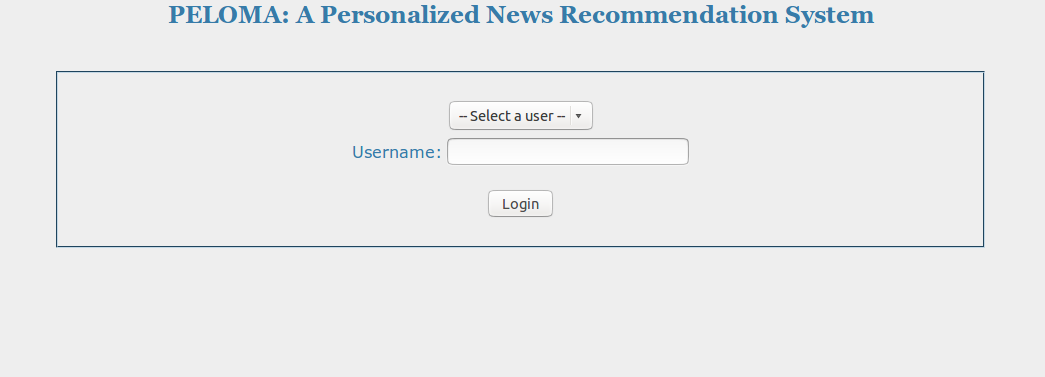
\includegraphics[scale=0.5]{static/figures/peloma/login.png}}
    \caption{Είσοδος χρήστη στο σύστημα.}
    \label{fig:inter01}
\end{figure} 

\begin{figure}[!ht] \centering
\centerline{
    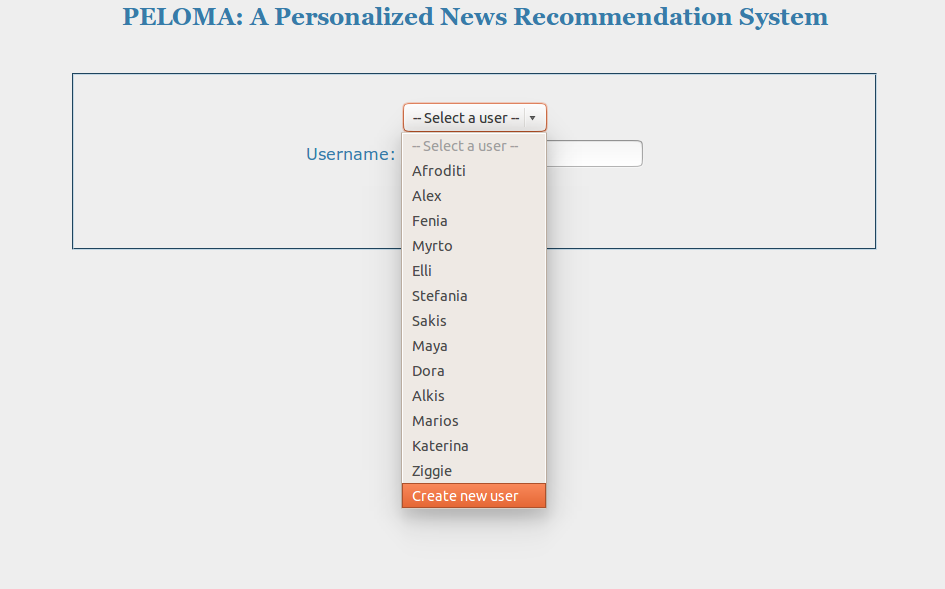
\includegraphics[scale=0.47]{static/figures/peloma/login2.png}}
    \caption{Είσοδος χρήστη στο σύστημα.}
    \label{}
\end{figure} 

Αμέσως μετά τη σύνδεση στο σύστημα, ο χρήστης οδηγείται στην κεντρική σελίδα της εφαρμογής, 
μέσω της οποίας αποκτά πρόσβαση στα άρθρα που είναι αποθηκευμένα στη βάση δεδομένων. 
Στην επάνω δεξιά γωνία του συστήματος αναγράφεται το {\en {username}} του συνδεδεμένου χρήστη και 
παρέχεται κουμπί για την αποσύνδεσή του από το σύστημα. 
Κατά την αποσύνδεση, ο χρήστης οδηγείται στην αρχική φόρμα εισόδου στην εφαρμογή. \\

\begin{figure}[!ht] \centering
\centerline{
    
\includegraphics[scale=0.35]{static/figures/peloma/logout.png}}
    \caption{Κουμπί αποσύνδεσης από το σύστημα.}
    \label{}
\end{figure} 

Σε περίπτωση όπου ο χρήστης επιχειρήσει τη λήψη συστάσεων χωρίς να έχει διαβάσει κάποιο από τα άρθρα του συστήματος, 
εμφανίζεται σχετικό μήνυμα, ενημερώνοντάς τον πως πρέπει να διαβάσει τουλάχιστον ένα άρθρο από κάποια κατηγορία 
προκειμένου να δωθεί στο σύστημα η απαραίτητη είσοδος σχετικά με τις προτιμήσεις του. \\

\begin{figure}[!ht] \centering
\centerline{
    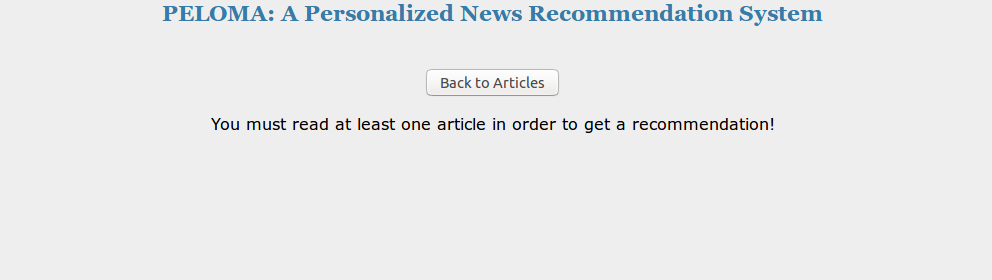
\includegraphics[scale=0.5]{static/figures/peloma/not.png}}
    \caption{Προσπάθεια λήψης συστάσεων πριν την ανάγνωση άρθρων.}
    \label{}
\end{figure} 

\newpage

Τα άρθρα παρουσιάζονται μέσω μιας λίστας στην οποία αναγράφονται το {\en {id}} της κατηγορίας, το {\en {id}} και ο τίτλος του κάθε άρθρου, 
ο οποίος τίτλος αποτελεί και {\en {link}} προς το πλήρες κείμενο. \\

\begin{figure}[!ht] \centering
\centerline{
    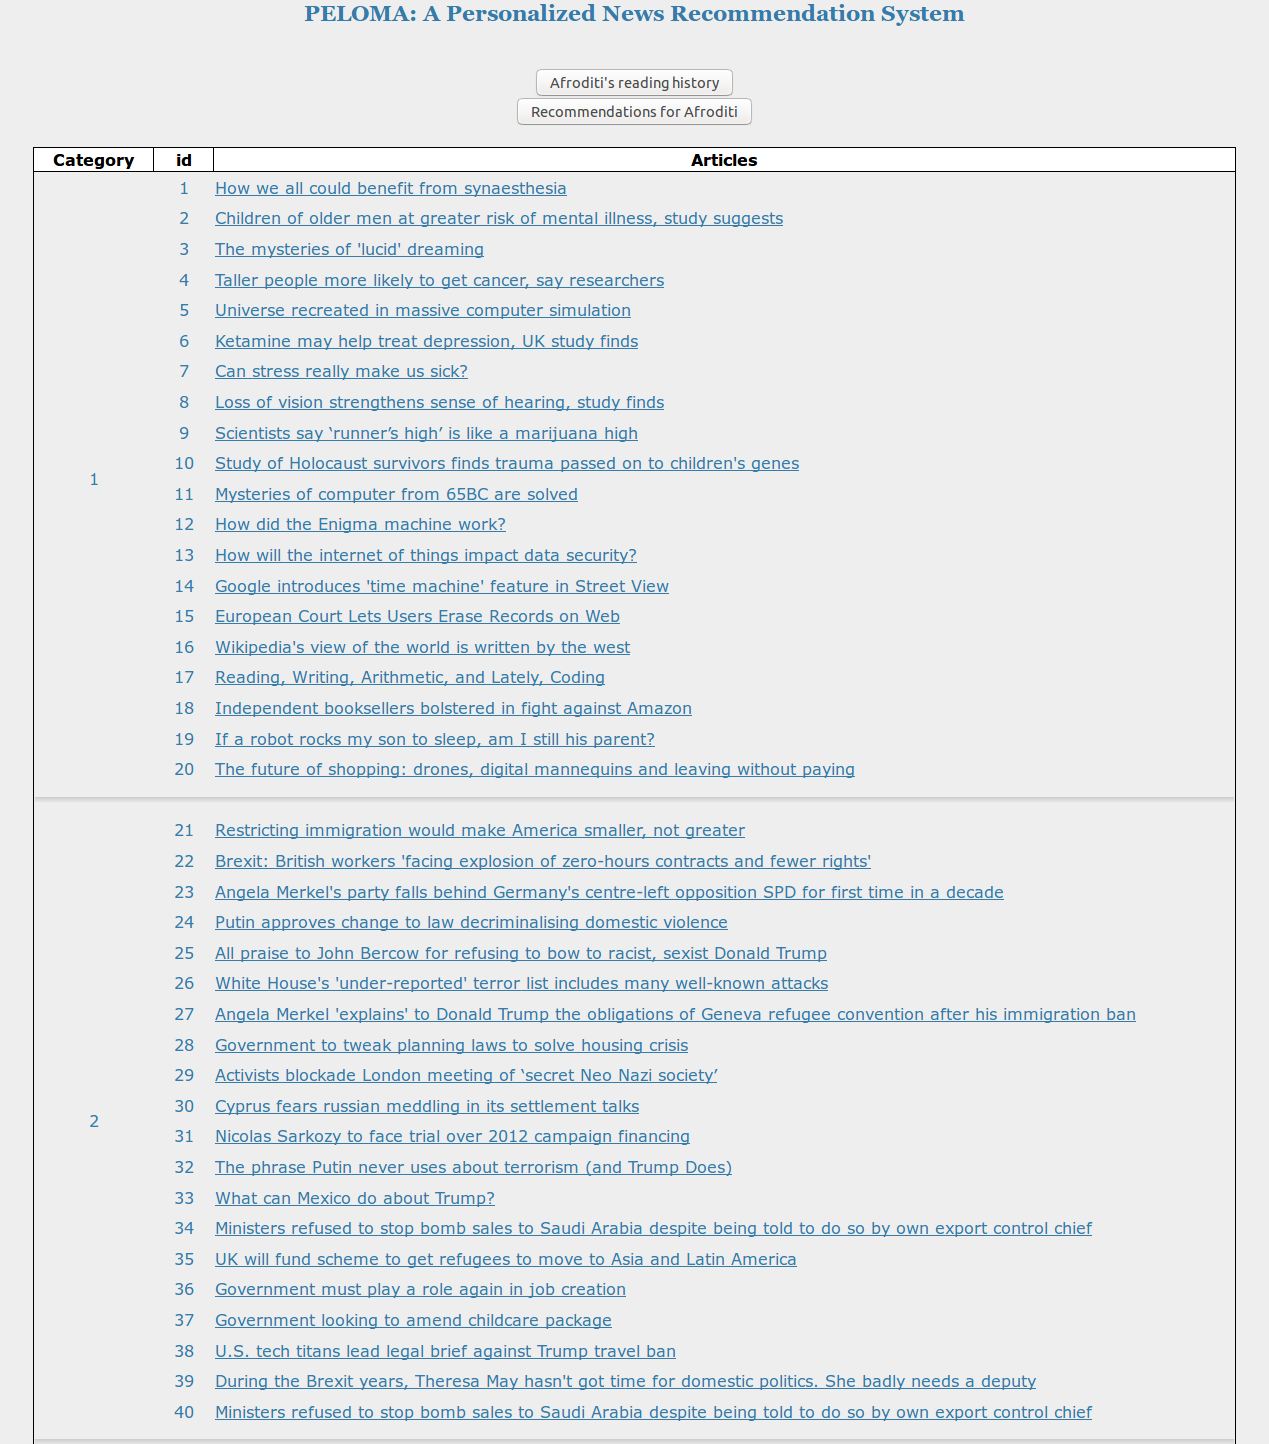
\includegraphics[scale=0.38]{static/figures/peloma/articles.png}}
    \caption{Προβολή λίστας άρθρων βάσης δεδομένων.}
    \label{}
\end{figure} 

\newpage

Παρακάτω βλέπουμε τη μορφή με την οποία παρουσιάζεται στο χρήστη το πλήρες κείμενο ενός άρθρου. 
Κατά το τέλος της ανάγνωσης ο χρήστης μπορεί να επιστρέψει στην αρχική λίστα άρθρων 
κάνοντας χρήση του κουμπιού \textit{{\en {Back to Articles}}} που βρίσκεται στο επάνω μέρος της σελίδας. \\

\begin{figure}[!ht] \centering
\centerline{
    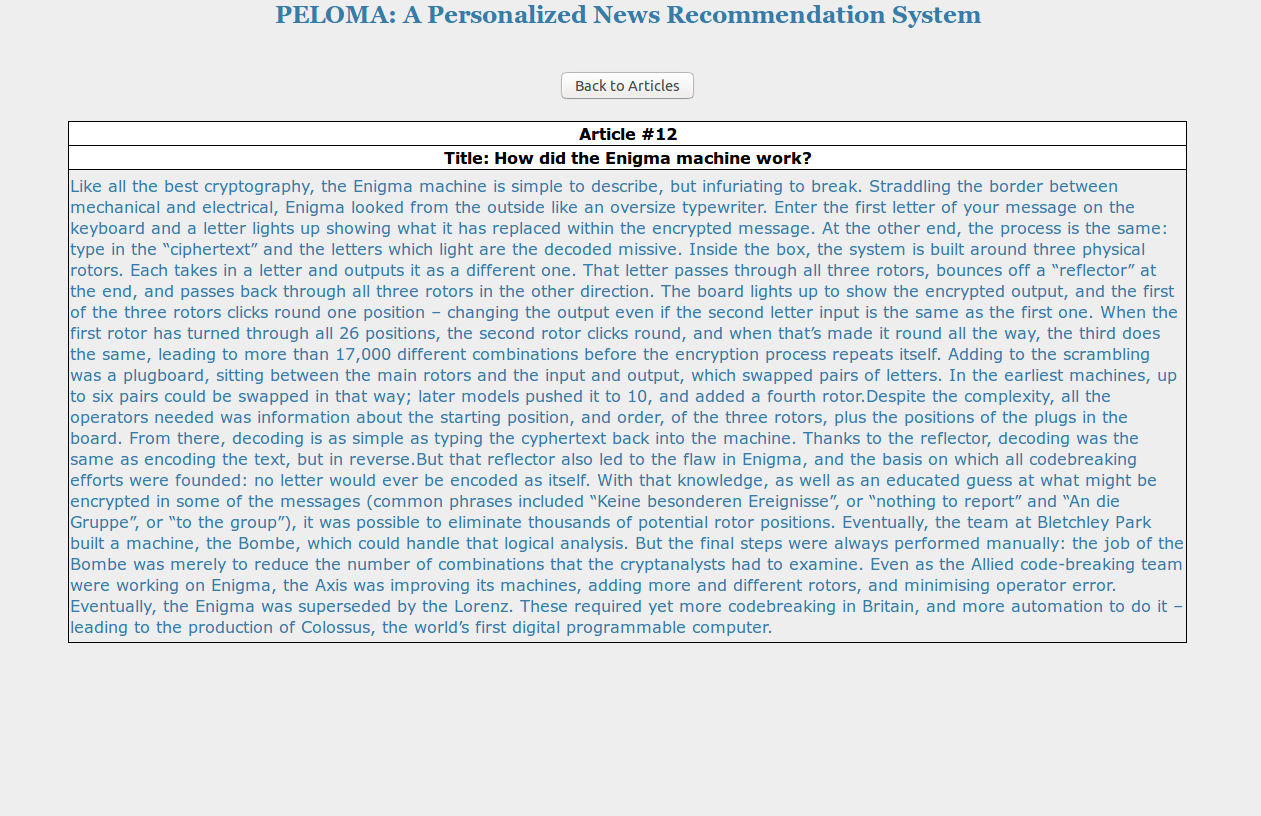
\includegraphics[scale=0.4]{static/figures/peloma/article.png}}
    \caption{Προβολή πλήρους κειμένου ενός άρθρου.}
    \label{}
\end{figure} 

\newpage

Κάθε άρθρο που αναγνώσθηκε αποθηκεύεται στη βάση δεδομένων στο ιστορικό ανάγνωσης 
του εν λόγω χρήστη. Ο χρήστης μπορεί ανά πάσα στιγμή να ενημερωθεί για τα άρθρα που έχει διαβάσει, 
μέσω του κουμπιού \textit{{\en {Reading history}}} που βρίσκεται στο επάνω μέρος της αρχικής σελίδας. \\

Αφού ο χρήστης περιηγηθεί μέσω της εφαρμογής διαβάζοντας άρθρα που τον ενδιαφέρουν, 
μπορεί να δεχθεί τις προσωποποιημένες συστάσεις άρθρων του συστήματος, 
πατώντας το κουμπί \textit{{\en {Recommendations for you}}} που βρίσκεται στο επάνω μέρος της σελίδας. 
Τότε, το σύστημα εμφανίζει μία λίστα με άρθρα που είναι πιθανό να τον ενδιαφέρουν, χωρισμένα σε κατηγορίες. 
Κάθε λίστα συστάσεων μπορεί να περιέχει άρθρα από το πολύ τρεις διαφορετικές κατηγορίες, 
δεδομένης της προτίμησης των χρηστών προς συγκεκριμένες κατηγορίες άρθρων. 
Για κάθε προτεινόμενο άρθρο αναγράφονται το {\en {id}} της κατηγορίας στην οποία ανήκει, 
το {\en {id}} και ο τίτλος του άρθρου, ο οποίος τίτλος αποτελεί και {\en {link}} προς το πλήρες κείμενο. \\
Το σύστημα εμφανίζει διαφορετικό αριθμό προτεινόμενων άρθρων ανά κατηγορία, 
ανάλογα με το ενδιαφέρον του χρήστη ως προς τη συγκεκριμένη θεματική ενότητα. \\

\begin{figure}[!ht] \centering
\centerline{
    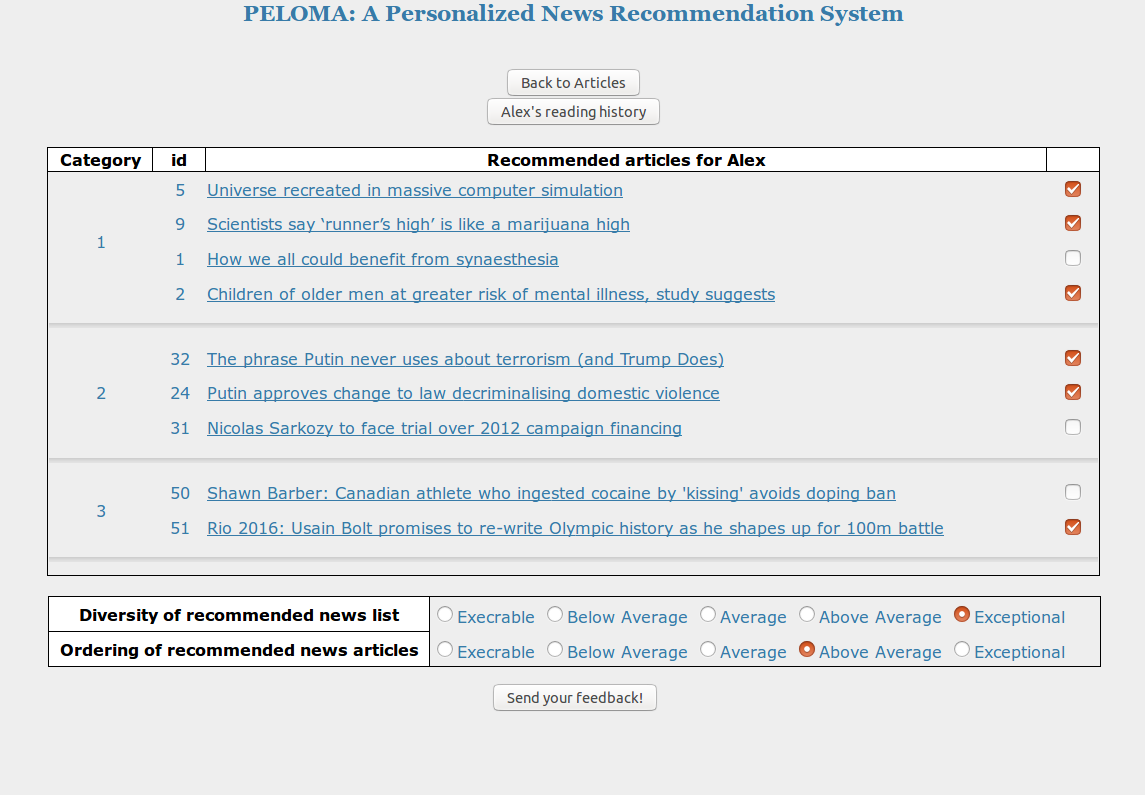
\includegraphics[scale=0.55]{static/figures/peloma/recommend.png}}
    \caption{Προβολή προσωποποιημένων συστάσεων.}
    \label{}
\end{figure} 

\newpage
Τέλος, ο χρήστης έχει την επιλογή να αξιολογήσει την ποιότητα των προσωποποιημένων συστάσεων του συστήματος. 
Μέσω των {\en {checkboxes}} που εμφανίζονται δίπλα στα άρθρα, 
μπορεί να επιλέξει τις προτάσεις του συστήματος που σχετίζονται πραγματικά με τα ενδιαφέροντά του. 
Ακριβώς κάτω από τη φόρμα συστάσεων μπορεί να αξιολογήσει το σύστημα 
τόσο ως προς την ποικιλία της λίστας συστάσεων, όσο και ως προς την κατάταξη των άρθρων της λίστας.\\

To {\en {feedback}} του χρήστη δίνεται στο σύστημα πατώντας το κουμπί {\en {Send your feedback!}}. \\
% \newpage

Ο αριθμός των άρθρων που ο χρήστης βρήκε ενδιαφέροντα αναγράφεται σε μορφή ποσοστού 
ως προς το συνολικό αριθμό προτεινόμενων άρθρων. \\

\begin{figure}[!ht] \centering
\centerline{
    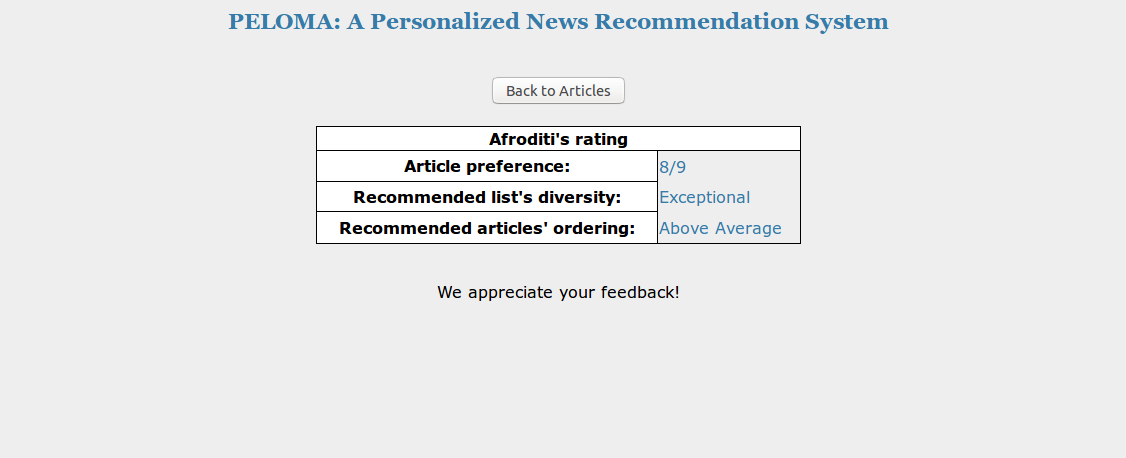
\includegraphics[scale=0.43]{static/figures/peloma/feedback2.png}}
    \caption{Αξιολόγηση συστήματος από το χρήστη.}
    \label{}
\end{figure} 

Ο χρήστης μπορεί είτε να αποσυνδεθεί από το σύστημα, είτε να συνεχίσει την ανάγνωση περισσότερων άρθρων, 
δεχόμενος εκ νέου συστάσεις. 